\section{Quantum Mechanics as a Framework}
\label{quantum_framework}
    \subsection{Linearity}
    \label{linearity}

    We begin with the fundamental elements of any physical theory: \textbf{equations of motion} and \textbf{dynamical variables}, which are related to our observations. Whenever we have a theory, we want to find these variables, because we can compare them with results from experiments.

    A \textbf{linear theory} means that given any two solutions to the equations of motion, the superposition of the solutions is also a solution.

    \begin{framedexpl} [Electromagnetism]
       The most famous linear theory is Maxwell's theory of electromagnetism. The linearity of electromagnetism allows electromagnetic fields to propagate without interfering. 
    \end{framedexpl}
    
    In Maxwell's theory, there are four dynamical variables: the electric field $\vec{E}$, magnetic field $\vec{B}$, charge $\rho$, and current density $\vec{J}$. Linearity implies:
    \begin{itemize}
    \item Given a solution $(\vec{E},\vec{B},\rho,\vec{J})$, we must have that $(\alpha\vec{E},\alpha\vec{B},\alpha\rho,\alpha\vec{J})$ is also a solution for all $\alpha\in\mathbb{R}$.
    \item Given two solutions $(\vec{E}_1,\vec{B}_1,\rho_1,\vec{J}_1)$ and $(\vec{E}_2,\vec{B}_2,\rho_2,\vec{J}_2)$, we must have that $(\vec{E}_1+\vec{E}_2,\vec{B}_1+\vec{B}_2,\rho_1+\rho_2,\vec{J}_1+\vec{J}_2)$ is also a solution.
    \end{itemize}
    
    A \textbf{linear equation} in one unknown is of the form $Lu=0$, where $u$ is an unknown and $L$ is a \textbf{linear operator}, which means it must satisfy two constraints:
    \begin{itemize}
        \item $L(au)=aLu$ for all $a\in\mathbb{R}$.
        \item $L(u_1+u_2)=Lu_1+Lu_2$ for all $u_1$ and $u_2$.
    \end{itemize}
    
    We see that given two solutions $u_1$ and $u_2$ to the linear equation, we can construct a general solution $\alpha u_1+\beta u_2$ for $\alpha,\beta\in\mathbb{R}$.

    A linear theory is much simpler than a nonlinear theory. For example, Maxwell's theory of electromagnetism (linear) is much simpler than Einstein's general relativity (nonlinear). 
    
    In fact, classical mechanics is highly nonlinear. Consider the equation for motion in 1 dimension with potential $V(x)$: $$m\frac{d^2x}{dt^2}=-V'(x).$$The problem is that the right-hand side may not be linear! For example the potential $V(x)=x^3$ makes $V'(x)$ go with $x^2$, which is nonlinear.

    \begin{framedexpl}[Three-body problem]
        The unsolvability of the three-body problem derives from the fact that classical mechanics is nonlinear.
    \end{framedexpl}

    \subsection{The Schrödinger Equation}\label{schrodinger}
    
    Fortunately, quantum mechanics is a linear theory! The dynamical variable is the \textbf{wavefunction} $\Psi(t,\vec{x})$. The equation of motion is the \textbf{Schrödinger Equation}: $$i\hbar\frac{\partial\Psi}{\partial t}=\hat{H}\Psi.$$Here, $\hat{H}$ is the \textbf{Hamiltonian}, a linear operator, and $\hbar$ is the \textbf{reduced Planck's constant}. The linear operator $L$ is given by $(i\hbar\frac{\partial}{\partial t}-\hat{H})$. The $i$ is, of course, the imaginary number $i=\sqrt{-1}$. The field $\mathbb{R}[i]$ is denoted $\mathbb{C}$ and is referred to as the \textbf{complex numbers}. 

    We define the \textbf{conjugate} of a complex number $z=a+bi$ as $z^*=a-bi$. Furthermore, the \textbf{norm} of $z$ is $|z|=\sqrt{a^2+b^2}$. This yields the important identity $|z|^2=zz^*$.
    
    \begin{framedthm}[Euler's formula]
        The complex number with norm 1 and angle $\theta$ to the real axis can be expressed as $$e^{ix}=\cos(x)+i\sin(x).$$
    \end{framedthm}
    
    For all physical systems, the wavefunction $\Psi$ must be a complex number. However, complex numbers cannot be directly measured. Instead, Max Born found that $|\Psi|^2$  is proportional to the probability of finding a particle in a given state.

    \begin{framedrmk*}[Simplicity]
        The linearity of quantum mechanics hints at an underlying simplicity. in fact, we will see throughout the semester that quantum mechanics is in some ways simpler and more beautiful than classical mechanics.
    \end{framedrmk*} 

    \section{Determinism}
    \label{determinism}
    \subsection{Photons}\label{photons}
      By Einstein's time, everyone knew from Maxwell's theories that light was a wave. However, Einstein posited that light was quantized into discrete particles, called \textbf{photons}. In classical mechanics, a particle is a point with well-defined mass, energy, position, and velocity. On the other hand, a particle in quantum mechanics is simply an indivisible packet. It does not necessarily have a defined mass or position or velocity.
    
    Einstein realized that the energy of a photon with frequency $\nu$ is given by $$E=h\nu.$$The frequency of light is related to its wavelength $\lambda$ by the equation $\nu\lambda=c$.
    
    \subsection{Polarization}\label{polar}
    
    A \textbf{polarizer} is an optical device that only transmits light that is linearly polarized in a certain direction. Consider a polarizer along the $x$-axis. Now let an electromagnetic wave linearly polarized at an angle $\alpha$ to the $x$-axis be sent through the polarizer. The resulting electric field is given by $$E=E_0\cos(\alpha)\hat{x}.$$Since the intensity of light is proportional to the square of the amplitude of the electric field, a fraction $\cos^2(\alpha)$ of the energy is transmitted through the polarizer.
    
    Now imagine the light beam consisting of a vast quantity of discrete photons. Then a fraction $\cos^2(\alpha)$ of the photons should be transmitted, while the rest should be absorbed. \textit{But the photons are identical, so classically, they should all behave the same!} In fact, the introduction of photons causes the loss of determinism.
    
    \begin{framedrmk*}[Troubles with photons]
        Einstein and his contemporaries were deeply troubled by the loss of determinism caused by photons. Einstein and others hypothesized that there are ``hidden variables,'' properties of photons that we can never know, that govern whether a photon gets transmitted. Alexander Bell famously proved that this does not resolve the difficulty, by showing that a ``Bell inequality'' would then hold. It was later experimentally shown to be false.
    \end{framedrmk*}
    
    We think of \textbf{states} of a particle as wavefunctions and vectors, which obey the same constraints of linearity. We represent a photon polarized in the $x$ direction using \textbf{Dirac notation}: $$\ket{\text{photon}:x}.$$We can similarly represent a photon polarized in the $y$ direction. By linearity, we can write the state of a photon polarized with angle $\alpha$ to the $x$-axis as $$\cos(\alpha)\ket{\text{photon}:x}+\sin(\alpha)\ket{\text{photon}:y}.$$

    \subsection{Superposition}\label{superposition}
    
    In classical mechanics, \textbf{superposition} is straightforward: the superposition of two electric fields, for example, is simply their sum --- another electric field. In quantum mechanics, superposition is very strange.

    A \textbf{Mach-Zehnder interferometer} is a device, invented in 1891, that demonstrates the effects of quantum superposition. In a Mach-Zehnder interferometer, a single beam of light is split; the two rays travel along symmetrical paths and meet at another beam splitter, where they undergo interference (see Figure \ref{mach-zehnder}).
    
    \begin{figure}[H]
        \centering
        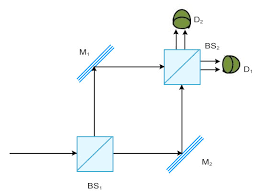
\includegraphics[width=0.5\linewidth]{resources/images/mach-zehnder.png}
        \caption{A Mach-Zehnder interferometer.}
        \label{mach-zehnder}
    \end{figure}
    
    We know that the first beam splitter will cause half of the photons at random to traverse each path. However, superposition can cause photons to travel down \textit{both} paths simultaneously.
    
    Consider sending photons individually into the interferometer. We observe experimentally that interference still occurs at the second beam splitter. Thus, each photon must be interfering \textit{with itself}.
    
    \begin{framedrmk*}[Interference of light]
        It may seem natural that the interference of light should be produced by two photons interfering. However, this cannot be the case! If two photons were to interfere destructively, it would violate the conservation of energy. Similarly, if two photons were to interfere constructively, the amplitude of the electric field would double, but the intensity would quadruple! This shows that light interference can only be the result of quantum superposition.
    \end{framedrmk*}
    
    Thus, a single photon in a Mach-Zehnder interferometer is a superposition of a photon in the upper path and a photon in the lower path.
    
    \begin{framedrmk*} [Superposition as a vector sum]
        A superposition of states can be thought of as the sum of the vectors representing the two states. Note that a vector can be written as the sum of two others in many different ways, and thus a state can be thought of as a superposition of others in many different ways. This will be very helpful later in the semester, as we try to understand states physically. 
    \end{framedrmk*} 
    
    Consider two states $\ket{A}$ and $\ket{B}$, and their superposition $\alpha\ket{A}+\beta\ket{B}$. Suppose a dynamical variable is always measured to be $a$ in state $\ket{A}$ and $b$ in state $\ket{B}$. Then measuring the variable in the superposition yields $a$ with probability proportional to $|\alpha|^2$ and $b$ with probability proportional to $|\beta|^2$. In fact, if $a$ is measured, the state becomes $A$, and the same is true with a measurement of $b$. That is, subsequent measurements will always yield the same result. Note that no \emph{intermediate} results are possible; only one of the two original values. 
    
    \begin{framedexpl}[Polarized photon]
        Consider the example of a photon in Section \ref{polar}. Here the two states are $\ket{\text{photon}:x}$ and $\ket{\text{photon}:y}$, and their superposition is given by $\cos(\alpha)\ket{\text{photon}:x}+\sin(\alpha)\ket{\text{photon}:y}$. The polarizer can be thought of as measuring the polarization of the photon. Then the probability of finding the photon polarized in the $x$ direction is proportional to $|\alpha|^2$, and the probability of finding it polarized in the $y$ direction is proportional to $|\beta|^2$.
    \end{framedexpl}

    We make the necessary physical assumption that superimposing a state with itself does not change any physics: $$\ket{A}\cong 2\ket{A}\cong -\ket{A}\cong i\ket{A}.$$We can see a physical interpretation of this fact using photons.

    \begin{framedexpl}[Polarized photon again]
        Consider a photon polarized in the state $$\alpha\ket{\text{photon}:x}+\beta\ket{\text{photon}:y}.$$This expression has two complex parameters: $\alpha$ and $\beta$. Due to our assumption, however, this state is physically equivalent to the state $$\ket{\text{photon};x}+\frac{\beta}{\alpha}\ket{\text{photon};y}.$$We can thus parameterize a general polarization state of a photon using a single complex parameter $\delta=\frac{\beta}{\alpha}$, or two real parameters. This is indeed physically accurate: a general polarization state of a photon is elliptical, with one variable describing the angle from the $x$-axis and another describing the eccentricity.
    \end{framedexpl}

    \subsection{Spin States}\label{spin_states}

    \textbf{Spin} is an intrinsic property of elementary particles that gives them angular momentum even when they are not rotating or orbiting. We measure spin along the $z$ axis; we find that all matter particles have spin $\frac{1}{2}$ and are either \textbf{spin up} or \textbf{spin down} in the $z$ direction. These are represented by the quantum states $$\ket{\uparrow;z}\text{ and }\ket{\downarrow;z}.$$We can then superimpose these two states to make the state $$\ket{\Psi}=\ket{\uparrow;z}+\ket{\downarrow;z}.$$Given a large number of electrons in this state, measuring the spin in the $z$ direction yields about 50\% spin up measurements and 50\% spin down measurements. 

    \begin{framedrmk*}[Hidden variable theories]
        Einstein believed that 50\% of the electrons are measured to be spin up because they were \textit{already} spin up; some hidden variable determined the spin of the electrons.

        It turns out that in the state $\ket{\Psi}$, 100\% of the electrons are spin up in the $x$ direction while Einstein's ensemble of 50\% spin up electrons and 50\% spin down electrons have the same proportion in the $x$ direction. It has been experimentally measured that all the electrons in the $\ket{\Psi}$ state are spin up in the $x$ direction.  
    \end{framedrmk*}

    \subsection{Entanglement}\label{entanglement}
    
    Consider two non-interacting particles. Suppose particle 1 can be in the states $\ket{u_1}$ and $\ket{u_2}$ and particle 2 can be in the states $\ket{v_1}$ and $\ket{v_2}$. Let the two particles be in the states $\ket{u_1}$ and $\ket{v_1}$, respectively. To represent both these states together, we write $$\ket{u_1}\otimes\ket{v_1}.$$On the other hand, the states of the particles could be more complex. In general, we can have the state $$(\alpha_1\ket{u_1}+\alpha_2\ket{u_2})\otimes(\beta_1\ket{v_1}+\beta_2\ket{v_2}),$$ which we can simply distribute as normal to get $$\alpha_1\beta_1\ket{u_1}\otimes\ket{v_1}+\alpha_2\beta_1\ket{u_2}\otimes\ket{v_1}+\alpha_1\beta_2\ket{u_1}\otimes\ket{v_2}+\alpha_2\beta_2\ket{u_2\otimes\ket{v_2}}.$$

    Now let us consider the following superposition of states: $$\ket{u_1}\otimes\ket{v_1}+\ket{u_2}\otimes\ket{v_2}.$$If this could be written as a product between a state of particle 1 and a state of particle 2, we would need $\alpha_1\beta_1=\alpha_2\beta_2=1$, while $\alpha_1\beta_2=\alpha_2\beta_1=0$. This is impossible; the state above is \textit{unfactorizable}. That is, the state of the first particle is dependent on the state of the second; we say that the particles are \textbf{entangled}.

    \begin{framedexpl}[Spin entanglement]
        Consider 2 spin $\frac{1}{2}$ particles, entangled in the quantum state $$\ket{\uparrow;z}_1\otimes\ket{\downarrow;z}_2+\ket{\downarrow;z}_1\otimes\ket{\uparrow;z}_2.$$
        This state is often used in an allegory with two friends named Alice and Bob, each of whom possesses one of the entangled particles. Even if Alice is several light-years away from Bob, any observation by Bob still instantly determines the state of Alice's particle. It was initially thought that this violated special relativity, which prohibits information from traveling faster than the speed of light. Luckily, it turns out that no information can be transmitted from Bob to Alice, or vice versa, in this way.
    \end{framedexpl}

    \section{Mach-Zehnder Interferometers}

    \subsection{Phase Shifters}
    
    Recall that in a Mach-Zehnder interferometer, a beam of light passes through a beam splitter. Both beams reflect off mirrors and recombine at a second beam splitter, which sends them to two different detectors. Additionally, we can put a device, such as a \textbf{phase shifter}, in between the first beam splitter and one of the mirrors.

    \begin{frameddefn}[Phase shifter]
        A \textbf{phase shifter} multiplies the probability amplitude by a fixed phase factor $\delta\in\mathbb{R}$. If an incoming wave has probability amplitude $\alpha$, the outgoing wave has probability amplitude $\alpha e^{i\delta}$. Since $|\alpha|=|\alpha e^{i\delta}|$, the phase shifter does not change the probability of finding the photon.
    \end{frameddefn}

    \begin{figure}[H]
        \centering
        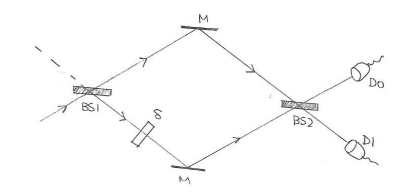
\includegraphics[width=0.7\linewidth]{resources/images/mach-zehnder-phase-shift.png}
        \caption{A Mach-Zehnder interferometer with a phase shifter.}
        \label{mach-zehnder-phase-shifter}
    \end{figure}

    We know that the state of a photon in a Mach-Zehnder interferometer is described by a wavefunction. We express the probability amplitudes of finding the photon in the upper beam and the lower beam by a column vector $\alpha\choose\beta$, where $\alpha,\beta\in\mathbb{C}$ reflect the probabilities of finding the photon in the upper and lower beams, respectively. Furthermore, we \textit{normalize} the probability amplitudes by requiring $|\alpha|^2+|\beta|^2=1$. 
    
    Note that the vector $1\choose0$ represents a photon in the upper beam, and $0\choose 1$ represents a photon in the lower beam. Thus, $\alpha\choose\beta$ is a superposition: ${\alpha\choose\beta} =\alpha {1\choose0}+ \beta {0\choose1}$.

    \subsection{Beam Splitters}

    We now consider the behavior of the beam splitters in detail. Suppose the beam splitter sends photons incident from above (with initial state $1\choose0$) to the state $s\choose t$, and photons incident from below (with initial state $0\choose1$) to the state $u\choose v$. Then we can represent the behavior of the beam splitter in general using linearity: an incident photon in state ${\alpha\choose\beta} =\alpha {1\choose0}+ \beta {0\choose1}$ is sent to the state $$\alpha{s\choose t}+\beta{u\choose v}={\alpha s+\beta u\choose \alpha t+\beta v}=\begin{pmatrix}
      s & u\\ 
      t & v
    \end{pmatrix}{\alpha\choose\beta}.$$Thus, the beam splitter can be completely represented by the 2x2 matrix with entries $s,t,u,$ and $v$, and we will say a beam splitter is equal to its matrix. In practice, the values of the coefficients are determined by the manufacturer. 
    
    \begin{framedrmk*}[Possible beam splitters]
        A beam splitter can be constructed if and only if acting on a normalized photon state always produces a normalized photon state. 
    \end{framedrmk*}
    
    In a \textbf{balanced beam splitter}, the probability that a photon is transmitted is always exactly $\frac{1}{2}$; that is, $|s|^2=|t|^2=|u|^2=|v|^2=\frac{1}{2}$. There are infinitely many complex numbers that satisfy this. However, let's suppose $s=t=u=v=\frac{\sqrt{2}}{2}$ and try acting on the normalized state $\sqrt{2}/{2}\choose \sqrt{2}/{2}$. Carrying out the matrix product yields $1\choose1$, which is not normalized.
    
    What if we instead try setting $v=-\frac{\sqrt{2}}{2}$? Carrying out the product $(\begin{smallmatrix}  s & u\\   t & v\end{smallmatrix}){\alpha\choose\beta}$ gives $\frac{1}{\sqrt{2}}{\alpha+\beta\choose \alpha-\beta}$. Finding the norm of this vector, we see that $$\frac{1}{2}|\alpha+\beta|^2+\frac{1}{2}|\alpha-\beta|^2=\frac{1}{2}[(\alpha+\beta)(\alpha^*+\beta^*)+(\alpha-\beta)(\alpha^*-\beta^*)].$$Note that the $\alpha\beta^*$ and $\beta\alpha^*$ terms vanish! We are left with $$\alpha\alpha^*+\beta\beta^*=|\alpha|^2+|\beta|^2=1.$$Thus, this is a valid balanced beam splitter! In fact, there is more than one possible matrix that satisfies these conditions. Specifically, the beam splitters $$BS_1=\frac{1}{\sqrt{2}}\begin{pmatrix}
      1 & 1\\ 
      1 & -1
    \end{pmatrix},\:\: BS_2=\frac{1}{\sqrt{2}}\begin{pmatrix}
      -1 & 1\\ 
      1 & 1
    \end{pmatrix}$$are both valid.

    \subsection{Experiments}
    
    Suppose we construct a Mach-Zehnder interferometer with these beam splitters: $$BS_1=\frac{1}{\sqrt{2}}\begin{pmatrix}
      1 & 1\\ 
      1 & -1
    \end{pmatrix},\:\: BS_2=\frac{1}{\sqrt{2}}\begin{pmatrix}
      -1 & 1\\ 
      1 & 1
    \end{pmatrix}.$$We send a photon with state $\alpha\choose\beta$ into the device; it passes through both beam splitters in sequence before exiting. Thus, the output state of the photon is $$(BS_2)(BS_1){\alpha\choose\beta}={\beta\choose -\alpha}.$$
    We now perform an experiment. Let us input a photon with state $0\choose1$. Then it should output in the state $1\choose 0$, so it should always hit the upper detector. 
    
    \begin{framedquest*}[What actually happened to the photon?]
        The photon split in the first beam splitter and recombined in the second. From both beams come some complex probability of transmission and reflection. The transmission from the top and reflection from the bottom interfered to give 0, while the transmission from the bottom and reflection from the top interefered to give 1.
    \end{framedquest*}

    Now we perform a slightly different experiment. This time, we place a block of concrete in between the first beam splitter and the bottom mirror. 

    \begin{figure}[H]
        \centering
        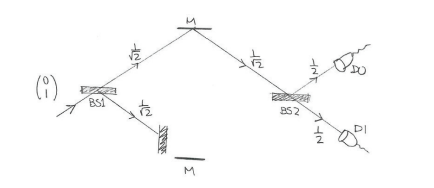
\includegraphics[width=0.7\linewidth]{resources/images/mach-zehnder-concrete.png}
        \caption{A Mach-Zehnder interferometer with a concrete block in the bottom path.}
        \label{mach-zehnder-concrete}
    \end{figure}
    
    We can no longer use the formula above, which was derived assuming both paths were possible. Instead, we must carry out the calculation from scratch. Suppose we send in a photon of state $0\choose 1$. Then the state after the first beam splitter is $$(BS_1){0\choose1}={\frac{1}{\sqrt{2}}\choose\frac{1}{\sqrt{2}}}.$$However, the bottom path is blocked. Thus, the input to the second beam splitter is only the first component: $\frac{1}{\sqrt{2}}\choose0$. Then the output is $$(BS_2){\frac{1}{\sqrt{2}}\choose0}={\frac{1}{2}\choose\frac{1}{2}}.$$There is a 50\% chance that the photon gets blocked, as expected. However, if the photon makes it through, there is a 50/50 chance of observing the photon in the upper or lower detector! Recall that without the concrete block, none of the photons reach the bottom detector.

    \subsection{Elitzur-Vaidman Bombs}
    
    An \textbf{Elitzur-Vaidman bomb} is a bomb triggered by a photon detector tube passing through the bomb. If the detector detects a photon, the bomb explodes. However, if the bomb is defective, the photon is transmitted normally. The question, which was posed by Avshalom Elitzur and Lev Vaidman in 1993, is the following: 

    \begin{framedquest*}[Elitzur-Vaidman bombs]
        Can we decide if an Elitzur-Vaidman bomb is defective without detonating it?
    \end{framedquest*}
    
    This seems obviously impossible, and indeed it is, using classical physics. However, quantum mechanics gives us an unexpected solution by embedding an Elitzur-Vaidman bomb into a Mach-Zehnder Interferometer.
    
    \begin{figure}[H]
        \centering
        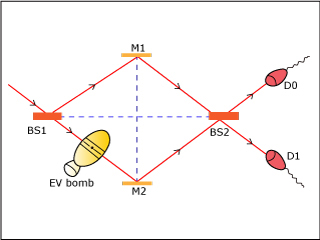
\includegraphics[width=0.5\linewidth]{resources/images/ev-bomb.png}
        \caption{A Mach-Zehnder interferometer with an Elitzur-Vaidman bomb.}
        \label{ev-bomb}
    \end{figure}
    
    We input a photon in the $0\choose1$ state. Suppose the bomb is defective, so the device behaves just like a normal interferometer. Then we can make the following table of possible outcomes and probabilities:

    \begin{center}
        \begin{tabular}{|c|c|}
            \hline
            \textbf{Outcome} & \textbf{Probability} \\
            \hline
            Photon to $D_0$ & 1   \\
            Photon to $D_1$ & 0   \\
            Bomb explodes   & 0   \\
            \hline
        \end{tabular}       
    \end{center}

    On the other hand, suppose the bomb is functional. Then any photon that passes along the bottom path gets absorbed and causes a detonation, so the device behaves like a blocked interferometer. Now our table looks like this:
    
    \begin{center}
        \begin{tabular}{|c|c|}
            \hline
            \textbf{Outcome} & \textbf{Probability} \\
            \hline
            Photon to $D_0$ & $1/4$   \\
            Photon to $D_1$ & $1/4$  \\
            Bomb explodes   & $1/2$  \\
            \hline
        \end{tabular}       
    \end{center}
    
    Note that $\frac{1}{4}$ of the time with a functional bomb, the photon is observed by $D_1$, whereas this never happens with a defective bomb! Thus, if we observe a photon at $D_1$, we know the bomb works without denotating it!
    
    \begin{framedrmk*}[Improvements]
       Is a $50\%$ chance that your lab explodes too high? It's been experimentally proven that this setup can be improved to decrease the probability of detonation arbitrarily low.
    \end{framedrmk*}